\chapter{State of the Art}

% ---- Figure placeholder (remove once real images are added) ----
\providecommand{\figplaceholder}[1]{%
    \fbox{\parbox[c][6cm][c]{0.85\textwidth}{\centering\texttt{#1}}}%
}


\label{chap:state_of_the_art}

\section{Introduction}
\label{sec:intro}

The transition from localized, physical co-location to distributed, hybrid work environments has transformed the landscape of collaborative knowledge work. Ideation, problem decomposition, and consensus building---traditionally carried out around physical whiteboards with adhesive notes---increasingly rely on digital collaborative environments. However, while commercial collaborative whiteboards provide shared visual surfaces, distributed teams frequently experience severe cognitive hurdles. Participants face cognitive overload from unstructured information sprawl, social loafing, evaluation apprehension, and anchoring biases that limit ideation breadth. Furthermore, transitioning from a divergent brainstorm of dozens of disparate thoughts to a structured, convergent action plan requires tedious manual synthesis.

This academic integration project, titled \textit{``Design and Implementation of an AI-Powered Collaborative Brainstorming Platform: MindSpark''}, investigates the convergence of real-time collaborative web architectures and modern artificial intelligence (AI). The central objective is to design a platform that not only provides low-latency, multi-user visual synchronization, but also integrates Generative AI and Large Language Models (LLMs) to actively assist ideators during both divergent expansion and convergent prioritization.

To establish a solid academic and technical foundation, this chapter presents an exhaustive review of the state of the art across four core pillars:
\begin{enumerate}
    \item \textbf{Collaborative Platforms and Ideation Dynamics:} Analyzing psychological mechanisms of group ideation, real-time web synchronization architectures, and an empirical comparative study benchmarking industry platforms against the current MindSpark prototype.
    \item \textbf{Generative AI and Large Language Models:} Reviewing transformer foundations, semantic embeddings, target AI-assisted brainstorming capabilities, prompt engineering paradigms, and the confirmed multi-tier AI microservice architecture.
    \item \textbf{SaaS Monetization and Resource Governance:} Examining architectural patterns for multi-tenant isolation, subscription lifecycles, rate limiting, and token budget governance essential for production viability.
    \item \textbf{Methodological Synthesis:} Connecting academic findings to the technical boundaries and development trajectory of the MindSpark platform.
\end{enumerate}

Throughout this chapter, a strict distinction is preserved between established theoretical principles, commercial implementations, the verified baseline of the MindSpark codebase, and target features confirmed for future realization.


\section{Collaborative Platforms \& Digital Brainstorming}
\label{sec:collab_platforms}

\subsection{Principles of Collaborative Ideation}
\label{subsec:ideation_principles}

The process of collaborative problem-solving is fundamentally grounded in cognitive and organizational psychology. In his seminal work on human intelligence, Guilford~\cite{guilford1956structure} established the operational distinction between \textit{divergent thinking} and \textit{convergent thinking}:
\begin{itemize}
    \item \textbf{Divergent Thinking:} The cognitive phase characterized by exploring a broad problem space, generating a high volume of varied perspectives, and suspending critical judgment. The metric of success is fluency, cognitive flexibility, and novelty.
    \item \textbf{Convergent Thinking:} The subsequent analytical phase where ideas are categorized, filtered, critically evaluated, and synthesized into a structured outcome or actionable decision.
\end{itemize}

Building on these foundations, Alex Osborn~\cite{osborn1953applied} formulated the principles of structured brainstorming, emphasizing four procedural rules: (1) defer judgment, (2) encourage unconventional ideas, (3) strive for quantity, and (4) combine and improve existing ideas. Despite its widespread adoption, empirical research by Diehl and Stroebe~\cite{diehl1987productivity} demonstrated that unguided face-to-face groups frequently suffer from significant productivity losses compared to nominal groups (individuals working in isolation whose outputs are pooled). These losses stem from three primary psychological inhibitors:
\begin{enumerate}
    \item \textbf{Production Blocking:} In verbal group meetings, only one individual can speak at any given moment. During this waiting period, other participants frequently forget their ideas or suppress them due to cognitive interference~\cite{diehl1987productivity}.
    \item \textbf{Evaluation Apprehension:} Individuals withhold unconventional ideas due to the fear of negative social judgment or peer criticism, which drives conformity toward safe, conservative suggestions~\cite{mullen1991productivity}.
    \item \textbf{Social Loafing and Free-Riding:} As group size increases, individual accountability declines, prompting individuals to exert less cognitive effort under the assumption that other group members will complete the task~\cite{karau1993social}.
\end{enumerate}

In addition to these inhibitors, group decision-making is severely vulnerable to \textit{anchoring bias}~\cite{tversky1974judgment}. When early ideas or prominent participants establish an initial reference point, subsequent thoughts gravitate disproportionately around that cognitive anchor, restricting the breadth of the ideation space.

Digital collaboration platforms address these barriers by providing parallelized input channels. Because participants can contribute sticky notes simultaneously on a digital canvas, production blocking is effectively eliminated. Furthermore, computer-supported idea generation enables anonymity mechanisms. As demonstrated by Connolly et al.~\cite{connolly1990idea}, decoupling ideas from personal identities substantially reduces evaluation apprehension, mitigates hierarchical intimidation, and reduces bandwagon voting biases, thereby fostering higher novelty and balanced group participation.

\subsubsection{The Anonymous Voting Challenge}
While digital whiteboards often provide visual voting indicators, implementing true anonymous voting presents a distinct technical challenge:
\begin{itemize}
    \item \textbf{Integrity vs. Anonymity:} A robust voting system must ensure each participant casts at most a defined number of ballots (e.g., one vote per idea) and retains the ability to retract or remove their vote.
    \item \textbf{The Inadequacy of Frontend Masking:} Merely omitting the user's name from client-facing JSON payloads does not provide true anonymity. If the underlying database persists a foreign key relation linking \texttt{user\_id} to \texttt{idea\_id}, the association is directly exposed to database administrators, audit logs, and any backend vulnerability.
    \item \textbf{Cryptographic Anonymity Solutions and Limitations:} Achieving unlinkable, verifiable voting requires cryptographic techniques such as blind signatures, zero-knowledge proofs, or salted cryptographic hashes ($H(\text{user\_id} \parallel \text{room\_salt})$). While salted hashing obfuscates direct identity linkage, hashing alone does not provide full cryptographic anonymity if the server retains access to both the salt and identity records, or if participation pools are small enough to allow correlation attacks. Robust anonymity architectures must separate eligibility verification from ballot persistence.
\end{itemize}


\subsection{Real-Time Web Communication}
\label{subsec:realtime_web}

Delivering a visual collaborative workspace where participants co-create on a shared virtual canvas requires robust network architectures capable of low-latency state synchronization. Over the evolution of the web, multiple paradigms have been developed to handle server-to-client updates.

\subsubsection{Evolution of Real-Time Communication Protocols}
Traditional web applications rely on the stateless, client-initiated \textbf{HTTP Request-Response} cycle. To simulate real-time updates, early collaborative tools adopted:
\begin{itemize}
    \item \textbf{Short Polling:} The client issues periodic HTTP GET requests (e.g., every 2 seconds). This introduces severe network overhead due to repetitive TCP connection handshakes and redundant HTTP headers, while introducing latency equal to the polling interval.
    \item \textbf{Long Polling (Comet):} The client opens an HTTP request that the server holds open until new data arrives or a timeout occurs. Once responded to, the client immediately re-establishes a new request. Although reducing idle traffic, long polling incurs substantial latency on high-frequency mutations and degrades under high concurrency.
    \item \textbf{Server-Sent Events (SSE):} Standardized by the WHATWG~\cite{whatwg_sse}, SSE provides a unidirectional, persistent HTTP stream (\texttt{text/event-stream}) allowing servers to push text data to browsers over standard HTTP/1.1 or HTTP/2. While well-suited for live dashboards and log streams, SSE is inherently unidirectional: client mutations must still be sent over separate HTTP POST/PUT requests, incurring multiple TCP streams.
    \item \textbf{The WebSocket Protocol (RFC 6455):} Standardized by the IETF~\cite{rfc6455}, WebSockets establish a persistent, bidirectional, full-duplex communication channel over a single TCP socket. After an initial HTTP Upgrade handshake, subsequent data exchanges occur via lightweight binary or text frames with only 2 to 10 bytes of framing overhead. WebSockets avoid redundant HTTP header exchanges, making them optimal for interactive multiplayer cursors and real-time canvas manipulations under reliable network conditions.
\end{itemize}

Figure~\ref{fig:rt-protocols} contrasts the message flow of these four paradigms.

\begin{figure}[htbp]
    \centering
    \figplaceholder{fig-realtime-protocols}
    % Replace the line above with:
    % 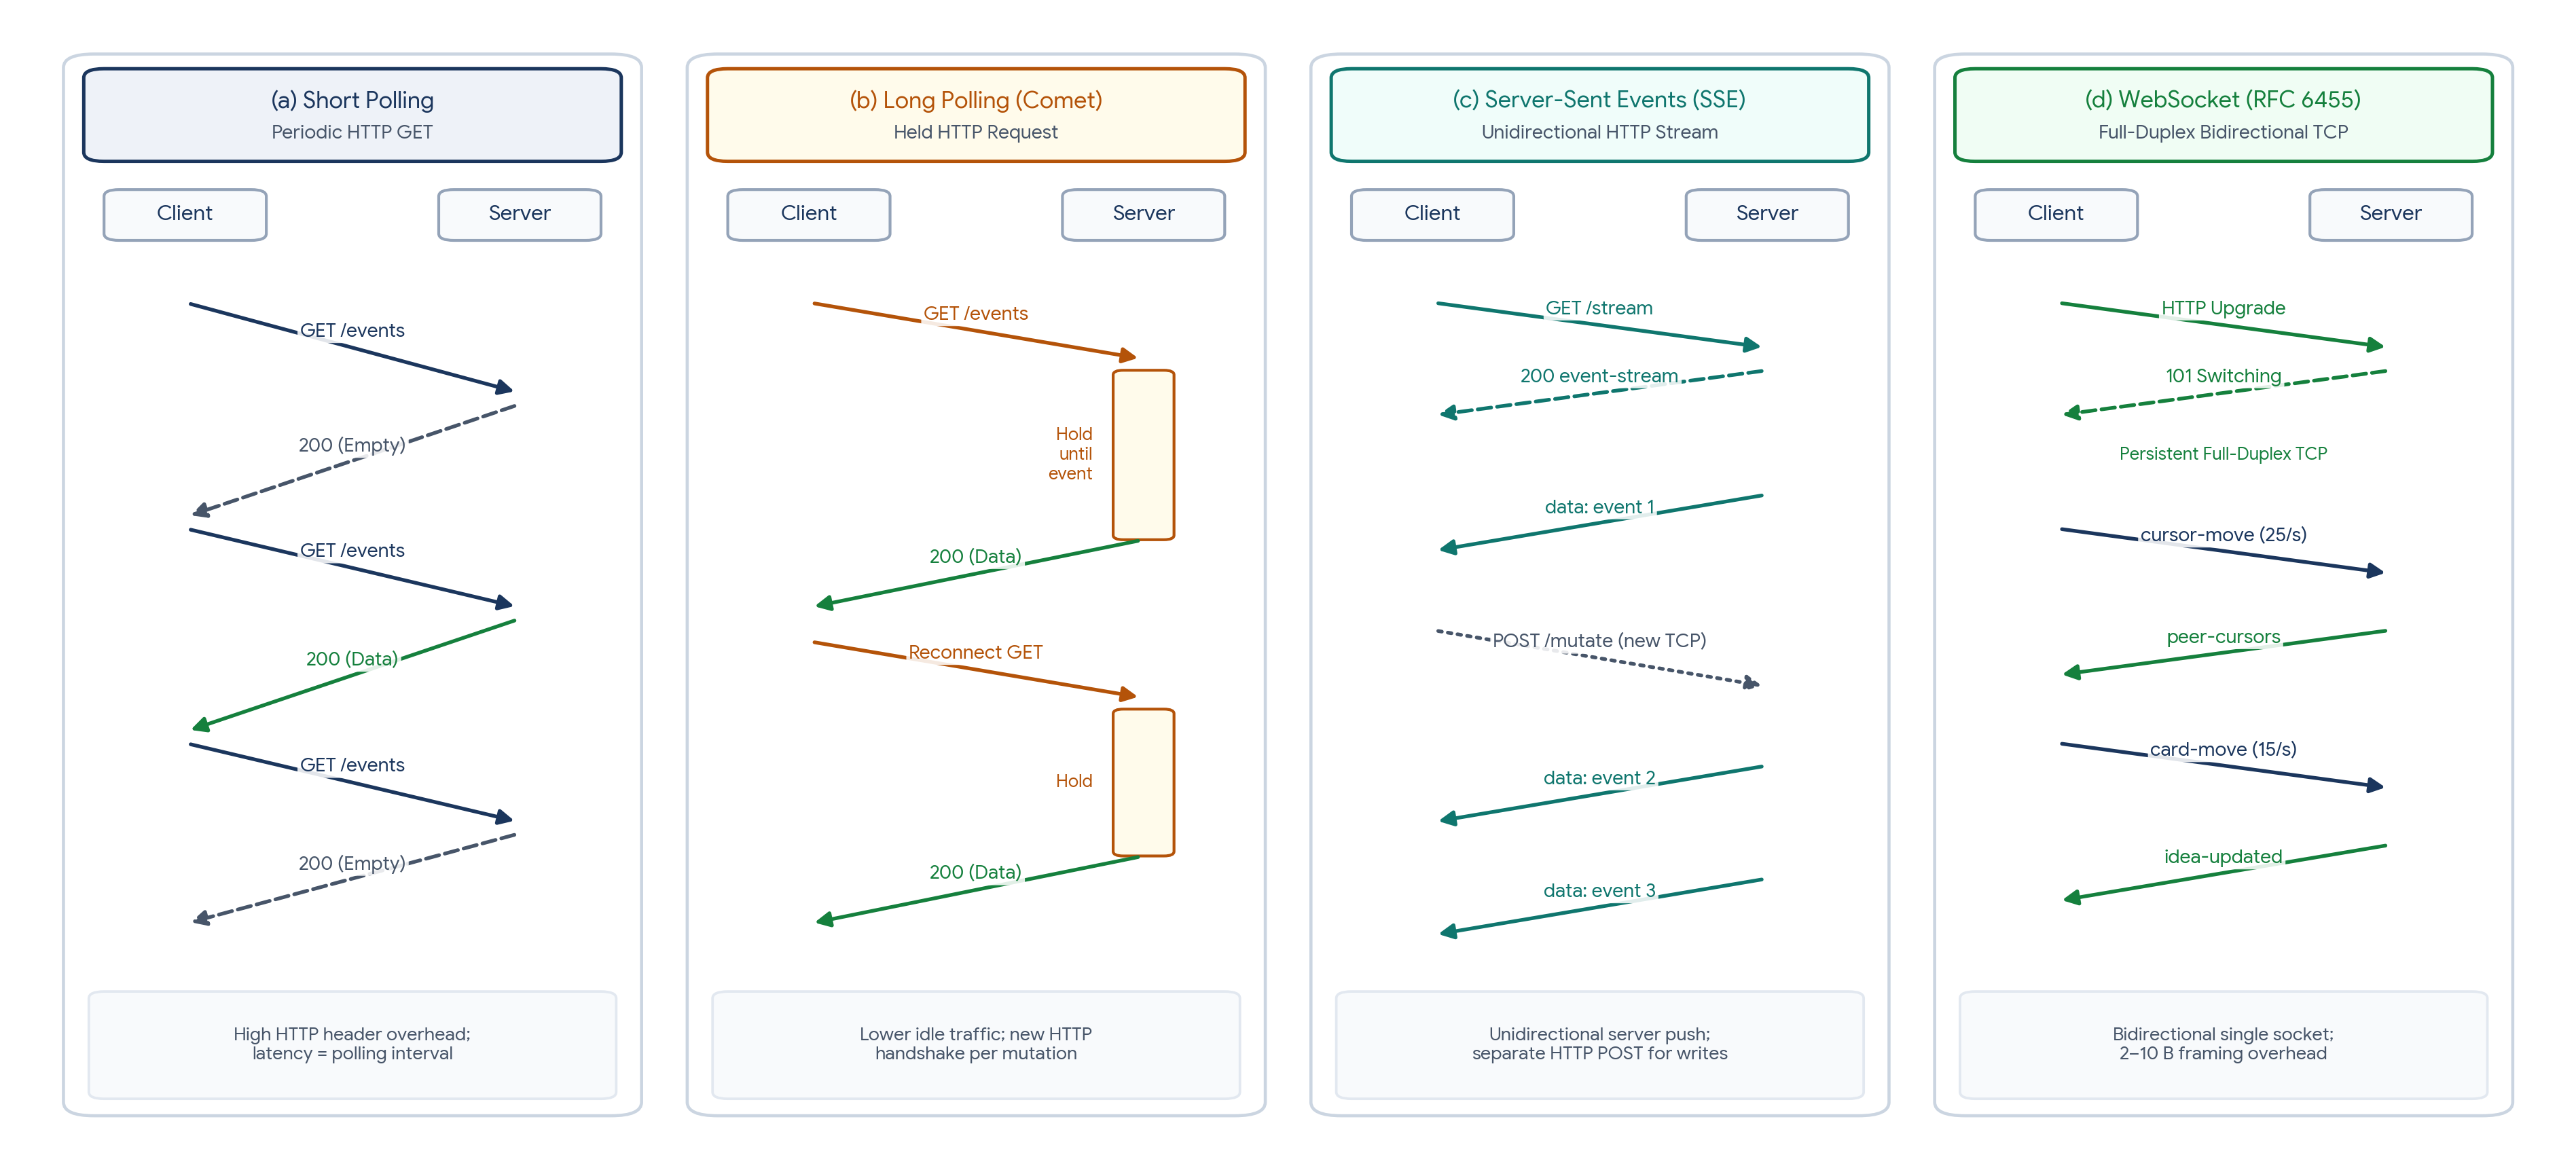
\includegraphics[width=0.9\textwidth]{fig-realtime-protocols}
    \caption{Message flow of short polling, long polling, Server-Sent Events, and WebSocket between a client and a server.}
    \label{fig:rt-protocols}
\end{figure}

\subsubsection{Publish-Subscribe Patterns and Room-Level Channel Isolation}
In multi-room collaboration environments, broadcasting every event globally to all connected clients is prohibitively inefficient. Systems employ the \textbf{Publish-Subscribe (Pub/Sub)} architectural pattern organized around room topics. Connected clients subscribe exclusively to their specific room identifier. Incoming mutations are dispatched solely to clients joined to that respective channel. While this ensures efficient real-time event filtering within the communication layer, it should be distinguished from comprehensive multi-tenant data isolation, which requires tenant partitioning across persistence layers and identity providers.

This room-scoped dispatching is illustrated in Figure~\ref{fig:pubsub-rooms}.

\begin{figure}[htbp]
    \centering
    \figplaceholder{fig-pubsub-room-isolation}
    % Replace the line above with:
    % 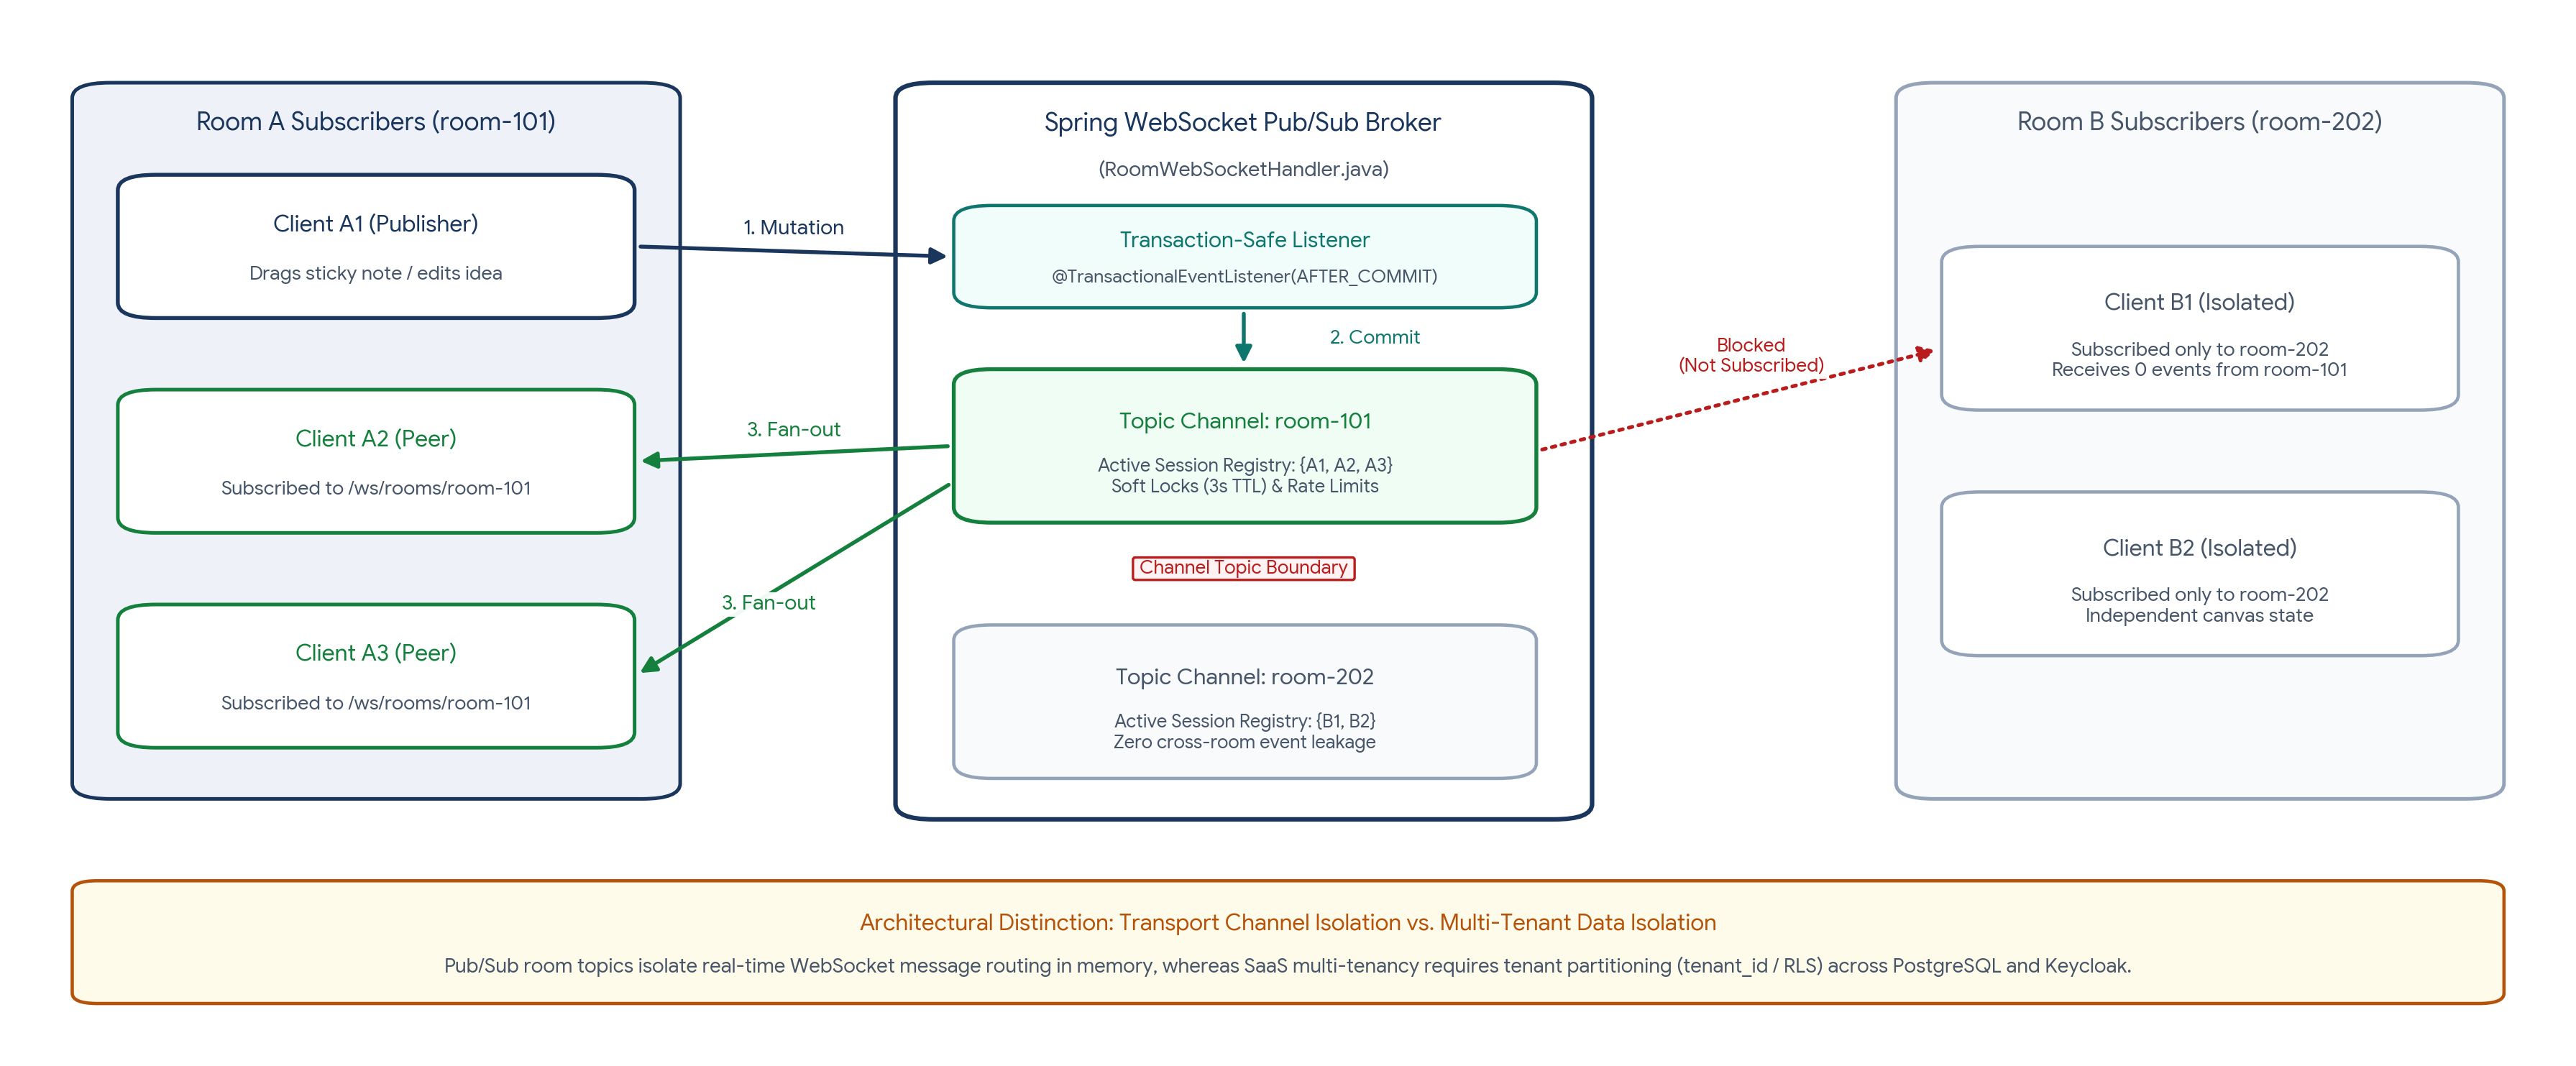
\includegraphics[width=0.9\textwidth]{fig-pubsub-room-isolation}
    \caption{Publish-Subscribe room-level channel isolation: mutations are dispatched only to clients subscribed to the originating room.}
    \label{fig:pubsub-rooms}
\end{figure}

\subsubsection{Multiplayer Presence and Live Cursor Synchronization}
Interactive whiteboard collaboration relies heavily on visual presence indicators to preserve spatial awareness and prevent duplicate actions. Live cursor synchronization transmits continuous pointer coordinates $(x, y)$ across participants. Because transmitting raw pixel coordinates at standard display refresh rates (60 to 144 Hz) would oversaturate network bandwidth, production systems implement three critical optimizations:
\begin{enumerate}
    \item \textbf{Coordinate Space Normalization:} Screen resolutions differ drastically across client devices. Cursors and objects must be mapped into a normalized virtual coordinate space (e.g., $X \in [0, 1000]$ and $Y \in [0, 500]$), enabling identical spatial rendering regardless of client viewport dimensions.
    \item \textbf{Client-Side Throttling:} Pointer movements are sampled and dispatched at a capped frequency (e.g., 20 to 25 updates per second), smoothing movements while preserving network stability.
    \item \textbf{Active Presence and Zombie Session Pruning:} Persistent connections can terminate abruptly without graceful TCP disconnects (e.g., laptop sleep, network loss). Servers must run automated background sweepers and periodic heartbeat pings to detect stale connections and evict ghost participants.
\end{enumerate}

\subsubsection{Concurrency Control and Transaction-Safe Broadcasting}
When multiple users manipulate the same visual element concurrently, race conditions and inconsistent states can emerge. High-throughput collaborative systems adopt distinct concurrency strategies depending on complexity:
\begin{itemize}
    \item \textbf{Operational Transformation (OT):} Transforms concurrent operation indices against each other to maintain linear document consistency, as utilized in collaborative text editors.
    \item \textbf{Conflict-Free Replicated Data Types (CRDTs):} Mathematically provable distributed data structures that achieve Strong Eventual Consistency without central coordination, but incur memory and metadata overhead.
    \item \textbf{Soft-Locking Mechanisms:} In spatial canvas environments, complex algorithmic transformation can often be avoided by utilizing distributed leases. Moving an object temporarily claims a short-lived exclusive lock (e.g., a 3-second sliding window lease), rejecting competing user interactions until released.
\end{itemize}

Furthermore, distributed architectures must guarantee \textbf{transaction-safe broadcasting}~\cite{spring_framework_doc}. If an event is broadcast over WebSockets before the underlying database transaction commits, a concurrent client reading the database might encounter race conditions or uncommitted data that could subsequently roll back. Decoupling event dispatching using application event listeners bound strictly to the \texttt{AFTER\_COMMIT} transaction phase ensures that clients only receive real-time notifications for durable state changes.

\subsubsection{Real-Time Implementation in the MindSpark Prototype}
The empirical audit of the MindSpark repository verifies that these real-time architectural principles are implemented in the current codebase:
\begin{itemize}
    \item \textbf{Full-Duplex WebSocket Engine:} MindSpark implements a native Spring WebSocket handler (\texttt{RoomWebSocketHandler.java}) communicating through Spring Cloud Gateway over \texttt{/ws/rooms/\{roomId\}}.
    \item \textbf{Coordinate Normalization \& Guards:} Cursor and object coordinates are mapped to a fixed virtual grid $[0, 1000] \times [0, 500]$ with boundary clamping on both the backend and Angular frontend (\texttt{idea-position-guard.ts}).
    \item \textbf{Adaptive Throttling:} Per-session rate limiters cap \texttt{cursor-move} at 25 events/sec, \texttt{stroke-points} at 20 events/sec, and \texttt{card-move} at 15 events/sec.
    \item \textbf{Soft Concurrency Locking:} Dragging an idea or vector drawing claims a 3-second sliding lock in memory (\texttt{heldObjects}), notifying peers with visual ``held by'' labels and preventing write collisions.
    \item \textbf{Transaction-Safe Event Dispatching:} In \texttt{RoomBroadcastEventListener.java}, domain mutations (\texttt{IdeaChangedEvent}, \texttt{DrawingChangedEvent}, \texttt{CategoryChangedEvent}) are annotated with \path|@TransactionalEventListener(phase = TransactionPhase.AFTER_COMMIT)|, preventing race conditions between persistence and real-time dispatch.
    \item \textbf{Automated Presence Sweeping:} A dedicated service (\texttt{PresenceSweeper.java}) executes an automated scheduled task every 5 seconds, evaluating client heartbeats (60s expiry + 10s grace) and gracefully removing disconnected members from the active room roster.
\end{itemize}


\subsection{Comparative Study Table}
\label{subsec:comparative_study}

To benchmark MindSpark within the broader ecosystem of visual collaboration tools, a systematic comparative study was conducted against four industry-leading platforms: \textbf{Miro}, \textbf{Mural}, \textbf{Klaxoon}, and \textbf{FigJam}. 

The comparison evaluates six core functional criteria:
\begin{enumerate}
    \item \textbf{Real-Time Cursors \& Presence:} Quality of multi-user spatial presence and viewport awareness.
    \item \textbf{Built-in Voting Mechanisms:} Native decision-making features and whether voting anonymity is enforced.
    \item \textbf{AI Idea Generation \& Expansion:} Ability of generative models to produce or elaborate brainstormed thoughts.
    \item \textbf{AI Semantic Clustering:} Automated affinity grouping and categorization of notes based on semantic similarity.
    \item \textbf{Action Plan \& Task Export:} Native conversion of brainstormed artifacts into structured project backlogs (e.g., Jira, Wrike, CSV).
    \item \textbf{Pricing Model \& Accessibility:} Commercial tier structures, billing intervals, and operational entry barriers.
\end{enumerate}

Data for commercial systems was gathered from verified official product and pricing documentation (accessed November 2026)~\cite{miro_pricing,mural_pricing,klaxoon_pricing,figjam_pricing}. Data for MindSpark is grounded strictly in the codebase audit.

\begin{table}[htbp]
\centering
\small
\setlength{\tabcolsep}{4pt}
\renewcommand{\arraystretch}{1.3}
\begin{tabularx}{\textwidth}{|>{\raggedright\arraybackslash}p{2.2cm}|*{4}{>{\raggedright\arraybackslash}X|}>{\raggedright\arraybackslash}p{3.2cm}|}
\hline
\textbf{Criterion} & \textbf{Miro}~\cite{miro_pricing} & \textbf{Mural}~\cite{mural_pricing} & \textbf{Klaxoon}~\cite{klaxoon_pricing} & \textbf{FigJam}~\cite{figjam_pricing} & \textbf{MindSpark (Audit)} \\ \hline
\textbf{Real-Time Cursors \& Presence} & 
Multi-user live cursors, participant following (``Follow me''). & 
Multi-user live cursors, facilitator ``Summon'', private mode. & 
Multi-user sticky notes, presenter board focus. & 
Multi-user live cursors, cursor chat, high-fives, live audio. & 
\textbf{Verified Implemented:} Normalized live cursors (25~Hz), soft locks (3s TTL), presence sweeper. \\ \hline
\textbf{Voting Mechanisms} & 
Dedicated Voting app: custom timers, multi-vote ballots, anonymous or open. & 
Facilitation Voting: ballot limits, secret ballots with reveal phase. & 
Integrated dot-voting, live polls, quizzes, and instant surveys. & 
Built-in Voting sessions: facilitator limits, timer, masked ballots. & 
\textbf{Verified Implemented (Non-Anonymous):} Upvote/downvote per idea. Voter ID linked in DB. \textit{Target: Cryptographic anonymous voting.} \\ \hline
\textbf{AI Idea Generation \& Expansion} & 
Miro AI: Generates mind maps, elaborates notes, summarizes topics. & 
Mural AI: Prompts brainstorming, mind mapping, and synthesis. & 
Board Setup Wizard: AI generated board frameworks and seed ideas. & 
FigJam AI: Generates templates, starter boards, and prompt expansions. & 
\textbf{Not Implemented (0\%):} Zero AI dependencies or generation endpoints found in code. \textit{Target: Confirmed ai-service microservice.} \\ \hline
\textbf{AI Semantic Clustering} & 
Automatic sticky note clustering by theme, keyword, and sentiment. & 
AI clustering by topic and sentiment; automated affinity mapping. & 
Automated categorization and synthesis of messy board notes. & 
Instant AI sort: groups unorganized sticky notes into themed clusters. & 
\textbf{Not Implemented (0\%):} Categorization is strictly manual via relational categories. \\ \hline
\textbf{Action Plan \& Task Export} & 
Converts stickies to Jira issues, Azure DevOps, or table summaries. & 
Exports to Jira, Asana, MS 365 Copilot, and structured PDFs. & 
Direct two-way sync with Jira \& Wrike; auto-generates action backlogs. & 
Converts sticky notes into tables, tasks, or Figma design elements. & 
\textbf{Not Implemented (0\%):} No export engine (PDF, CSV, Jira, or Markdown summary) exists. \\ \hline
\textbf{Pricing Model} & 
Free (\$0, 3 boards, 10 AI credits); Starter (\$8/member/mo annual); Business (\$20/member/mo annual, \$25 monthly); Enterprise. & 
Free (\$0, 3 murals); Team+ (\$9.99/user/\allowbreak mo annual, \$12 monthly); Business (\$17.99/user/\allowbreak mo annual); Enterprise. & 
Free (\$0, 1 open activity, max 5 participants); Starter (\$24.90/host/\allowbreak mo annual); Enterprise. & 
Free (\$0, 3 files); Collab Seat (\$3/mo); Dev Seat (\$12/mo); Full Seat (\$16/\allowbreak \$55/\allowbreak \$90/\allowbreak mo annual). & 
\textbf{Academic Prototype (Public Repo):} Single-tenant containerized environment. Zero billing or tier limits. \\ \hline
\end{tabularx}
\caption{Comparative Study: Commercial Collaboration Tools vs. MindSpark Prototype}
\label{tab:comparative_study}
\end{table}

\subsubsection{Analytical Synthesis of the Benchmark}
The comparative analysis reveals two critical insights:
\begin{enumerate}
    \item \textbf{Commercial Paywalls on AI Facilitation:} In commercial tools (Miro, Mural, Klaxoon), intelligent facilitation features---specifically semantic clustering, automated session summarization, and task decomposition---are restricted to paid subscription tiers or governed by metered credit allocations. Small teams, educational institutions, and open-source communities are frequently priced out of AI-augmented collaboration.
    \item \textbf{MindSpark's Strategic Opportunity:} The current MindSpark codebase provides a functional foundation for real-time collaboration, spatial synchronization, and concurrency control that mirrors the core mechanics of commercial canvases. However, it currently lacks all AI features and provides only non-anonymous voting. Developing native, open AI orchestration directly into this existing collaborative foundation represents the primary scientific and engineering contribution of this project.
\end{enumerate}


\section{Generative AI \& Large Language Models}
\label{sec:gen_ai}

\subsection{Generative AI \& LLMs}
\label{subsec:llm_foundations}

Artificial Intelligence has undergone a profound paradigm shift from discriminative models (which classify or predict based on input distributions) to \textbf{Generative AI}, which synthesizes novel, high-dimensional artifacts including text, code, and structured data. At the forefront of this revolution are \textbf{Large Language Models (LLMs)}.

\subsubsection{The Transformer Architecture}
Modern LLMs are built upon the \textbf{Transformer} architecture introduced by Vaswani et al.~\cite{vaswani2017attention}, extending the deep bidirectional representation foundations established by models such as BERT~\cite{devlin2019bert}. Unlike preceding recurrent neural network (RNN) or long short-term memory (LSTM) architectures that processed sequential tokens step-by-step, the Transformer relies entirely on the \textbf{Self-Attention Mechanism}:
\begin{equation}
    \text{Attention}(Q, K, V) = \text{softmax}\left(\frac{QK^T}{\sqrt{d_k}}\right)V
\end{equation}
Where $Q$, $K$, and $V$ represent the Query, Key, and Value matrices projected from token representations, and $d_k$ denotes the dimensionality of the key vectors. By computing attention scores between all tokens concurrently across multiple heads (Multi-Head Attention), Transformers capture long-range semantic dependencies, contextual nuances, and polysemy with exceptional parallel efficiency during training.

\subsubsection{Tokens, Context Windows, and Autoregression}
LLMs do not process raw text strings directly; input text is parsed into discrete sub-word segments termed \textbf{tokens} (typically $\approx 0.75$ words per token in English) using algorithms such as Byte-Pair Encoding (BPE). As demonstrated in autoregressive models such as GPT-3~\cite{brown2020language}, models operate by predicting the probability distribution of the next token $x_t$ conditioned on preceding tokens:
\begin{equation}
    P(x_1, x_2, \dots, x_T) = \prod_{t=1}^T P(x_t \mid x_1, \dots, x_{t-1})
\end{equation}
The \textbf{Context Window} defines the maximum sequence length (tokens) the model can ingest and attend to in a single forward pass. Recent LLM generations feature context windows ranging from 128,000 to over 1,000,000 tokens, enabling comprehensive ingestion of entire brainstorming sessions, room histories, and participant interactions.

\subsubsection{Vector Embeddings and Semantic Similarity}
While autoregressive LLMs excel at generation and reasoning, specialized transformer encoders (e.g., Sentence-BERT~\cite{reimers2019sentencebert}) map variable-length texts into fixed-size dense vector spaces $\mathbb{R}^d$ (typically $d \in [768, 1536]$). In this latent embedding space, semantic proximity corresponds directly to geometric distance. The similarity between two textual ideas $u$ and $v$ is quantified using \textbf{Cosine Similarity}:
\begin{equation}
    \text{CosineSimilarity}(u, v) = \frac{\mathbf{u} \cdot \mathbf{v}}{\|\mathbf{u}\|_2 \|\mathbf{v}\|_2}
\end{equation}
Dense embeddings provide the mathematical basis for deduplication, semantic clustering, and similarity retrieval in brainstorming sessions.


\subsection{AI Techniques for MindSpark}
\label{subsec:ai_techniques}

In the current baseline implementation, \textbf{no AI capabilities are implemented in the MindSpark repository}. This section formalizes the confirmed multi-tier provider strategy, microservice architecture, and proposed functionality targeted for subsequent implementation phases.

\subsubsection{Confirmed Multi-Tier AI Provider Strategy}
MindSpark's confirmed AI integration strategy employs a multi-tier cloud routing model designed to balance operational cost and low latency across distinct subscription tiers:
\begin{itemize}
    \item \textbf{Free Tier Routing (Google Gemini via OpenAI-Compatible Endpoint):}
    \begin{itemize}
        \item \textit{Primary Model:} \texttt{gemini-3.5-flash-lite}~\cite{google_gemini_models}. Optimized for ultra-low latency, cost efficiency, and high throughput, making it suitable for basic idea generation, drafting, and agentic query classification.
        \item \textit{Fallback Model:} \texttt{gemini-3.1-flash-lite}~\cite{google_gemini_models}. Latency-sensitive fallback model activated upon primary rate-limiting or service degradation.
    \end{itemize}
    \item \textbf{Premium Tier Routing (Groq LPU Hardware Inference):}
    \begin{itemize}
        \item \textit{Primary Model:} \texttt{openai/gpt-oss-120b}~\cite{groq_models_docs}. A 120-billion parameter open-weights Mixture-of-Experts (MoE) model executed on Groq's specialized Language Processing Unit (LPU) architecture for deep reasoning, complex semantic synthesis, and multi-idea trade-off analysis.
        \item \textit{Fallback Model:} \texttt{qwen/qwen3.8-27b}~\cite{groq_models_docs}. A 27-billion parameter dense multimodal model providing high-speed text processing and contextual reasoning fallback.
    \end{itemize}
\end{itemize}
Internal team benchmarks report target response times of approximately 0.8 seconds on the Groq Premium tier; however, this figure represents an internal team measurement under development conditions rather than an independently verified production benchmark. Both cloud providers will be accessed through standard OpenAI-compatible REST endpoints.

\subsubsection{Confirmed AI Microservice Architecture (\texttt{ai-service})}
Rather than relying on heavy abstractions (such as Spring AI or external Python/FastAPI microservices), the confirmed design specifies a dedicated Spring Boot microservice named \texttt{ai-service}:
\begin{itemize}
    \item \textbf{Ecosystem Homogeneity:} Preserves end-to-end consistency with the Java 21 / Spring Boot 4.1.1 backend stack, utilizing Spring Cloud Netflix Eureka for discovery and Spring Cloud Gateway for centralized edge routing (\texttt{lb://ai-service}).
    \item \textbf{Security Integration:} Natively integrates with Keycloak 26.2.4~\cite{keycloak_docs} OAuth2 Resource Server filters, validating JWT claims and enforcing role-based permissions (\texttt{ROLE\_USER}, \texttt{ROLE\_PREMIUM}).
    \item \textbf{Custom OpenAI-Compatible Client:} Implements a lightweight, custom HTTP client using Java's modern \texttt{RestClient} / \texttt{HttpClient}. This grants explicit granular control over per-attempt connect/read timeouts, total request timeouts, circuit breaking, and retry logic.
    \item \textbf{Autonomous Quota Management:} Maintains a dedicated PostgreSQL database instance to record daily token consumption, track per-user query quotas, and enforce reset windows independently of the core application database.
\end{itemize}

The overall request path is depicted in Figure~\ref{fig:ai-service-arch}.

\begin{figure}[htbp]
    \centering
    \figplaceholder{fig-ai-service-architecture}
    % Replace the line above with:
    % 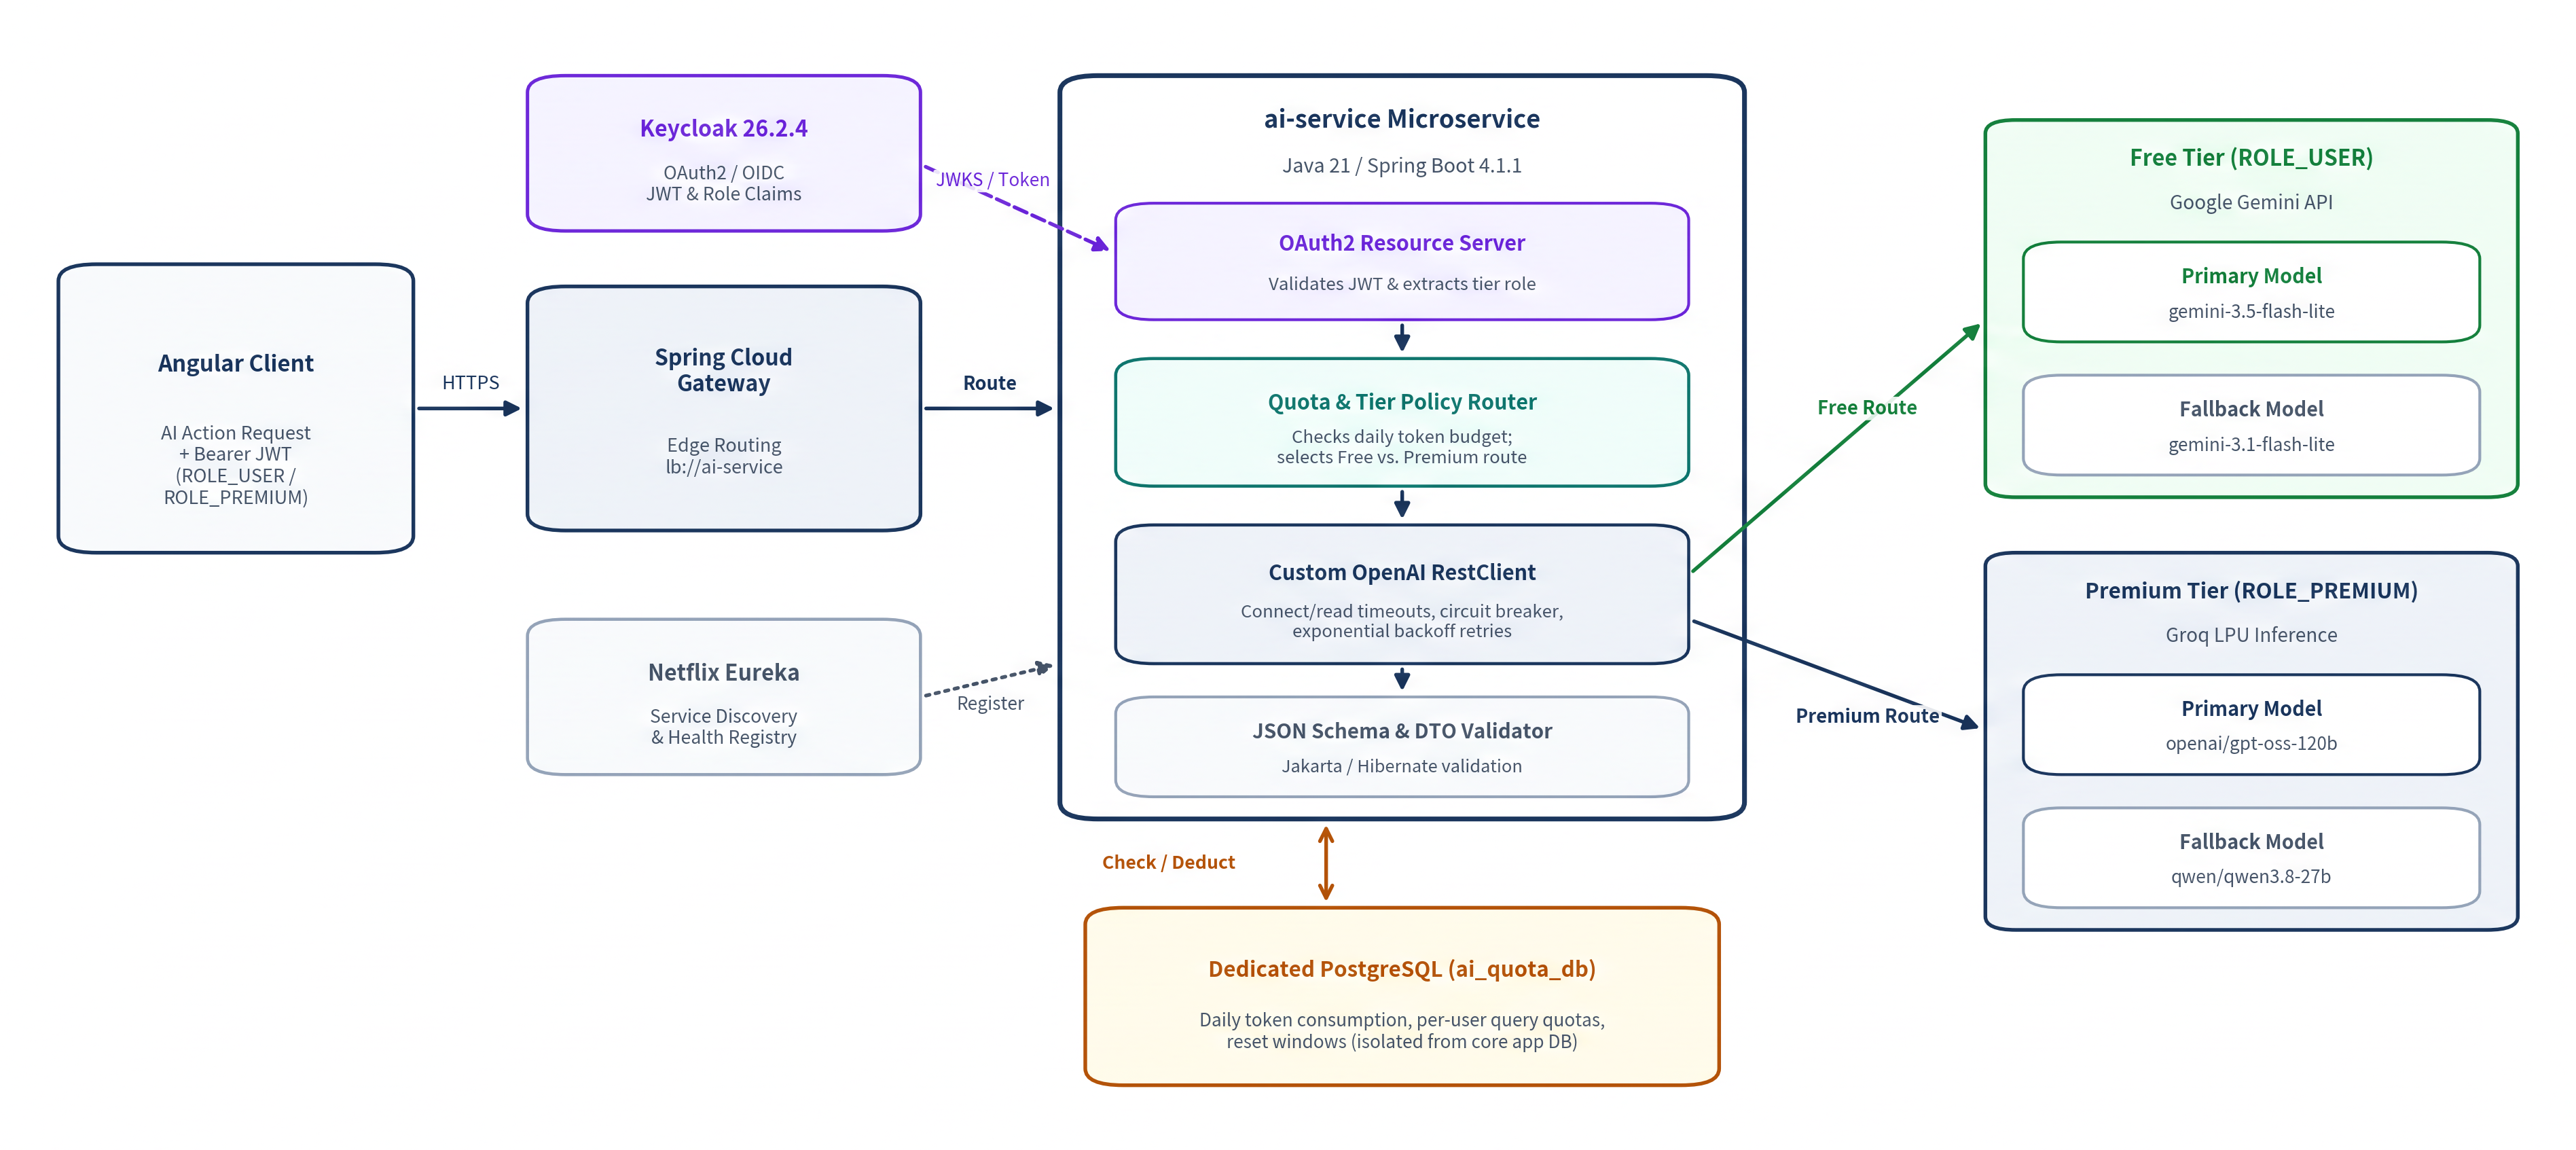
\includegraphics[width=0.9\textwidth]{fig-ai-service-architecture}
    \caption{Target architecture of the \texttt{ai-service} microservice within the MindSpark backend, including gateway routing, authentication, provider tiers, and quota storage.}
    \label{fig:ai-service-arch}
\end{figure}

\subsubsection{Target Brainstorming Capabilities}
The target functional capabilities planned for the \texttt{ai-service} include:
\begin{enumerate}
    \item \textbf{Topic-Based Idea Generation:} Generating starter ideas when participants encounter creative blocks.
    \item \textbf{Idea Expansion and Elaboration:} Assisting ideators in expanding brief notes into concrete concepts.
    \item \textbf{Semantic Clustering:} Grouping scattered sticky notes into thematic clusters using embedding clustering (e.g., DBSCAN~\cite{ester1996density}) or LLM zero-shot categorization.
    \item \textbf{Session Summarization:} Synthesizing active boards into structured Markdown overviews.
    \item \textbf{Risk and Assumption Detection:} Evaluating brainstormed concepts against feasibility and operational risk taxonomies.
    \item \textbf{Idea Comparison:} Generating structured matrices to compare competing solutions.
    \item \textbf{Action Plan Generation:} Decomposing prioritized ideas into assignable tasks with acceptance criteria.
\end{enumerate}


\subsection{Prompt Engineering \& Output Validation}
\label{subsec:prompt_engineering}

Integrating Large Language Models into a real-time web application requires a disciplined engineering pipeline to ensure predictable, structured, and safe outputs.

\subsubsection{Prompt Structuring and Context Injection}
A robust prompt pipeline consists of three distinct layers:
\begin{enumerate}
    \item \textbf{System Prompt:} Establishes the operational persona, behavioral constraints, safety boundaries, and output formatting rules (e.g., instructing the model to act as a design thinking facilitator and enforce JSON schemas).
    \item \textbf{Context Injection:} Extracting the room topic, category hierarchy, active sticky notes, and vote counts from PostgreSQL and serializing them into the prompt's context window.
    \item \textbf{User Prompt:} The immediate action requested by the participant (e.g., expanding an idea or clustering notes).
\end{enumerate}

To improve output quality and reasoning fidelity, techniques such as \textbf{Chain-of-Thought (CoT)} prompting~\cite{wei2022chain} instruct the model to decompose complex problems into intermediate reasoning steps. However, in automated web microservices, exposing lengthy natural-language reasoning tokens introduces unnecessary latency and parsing overhead; system design must prioritize validated, structured outputs over unconstrained narrative text.

Figure~\ref{fig:prompt-pipeline} summarizes the complete pipeline from user action to broadcast.

\begin{figure}[htbp]
    \centering
    \figplaceholder{fig-prompt-pipeline}
    % Replace the line above with:
    % 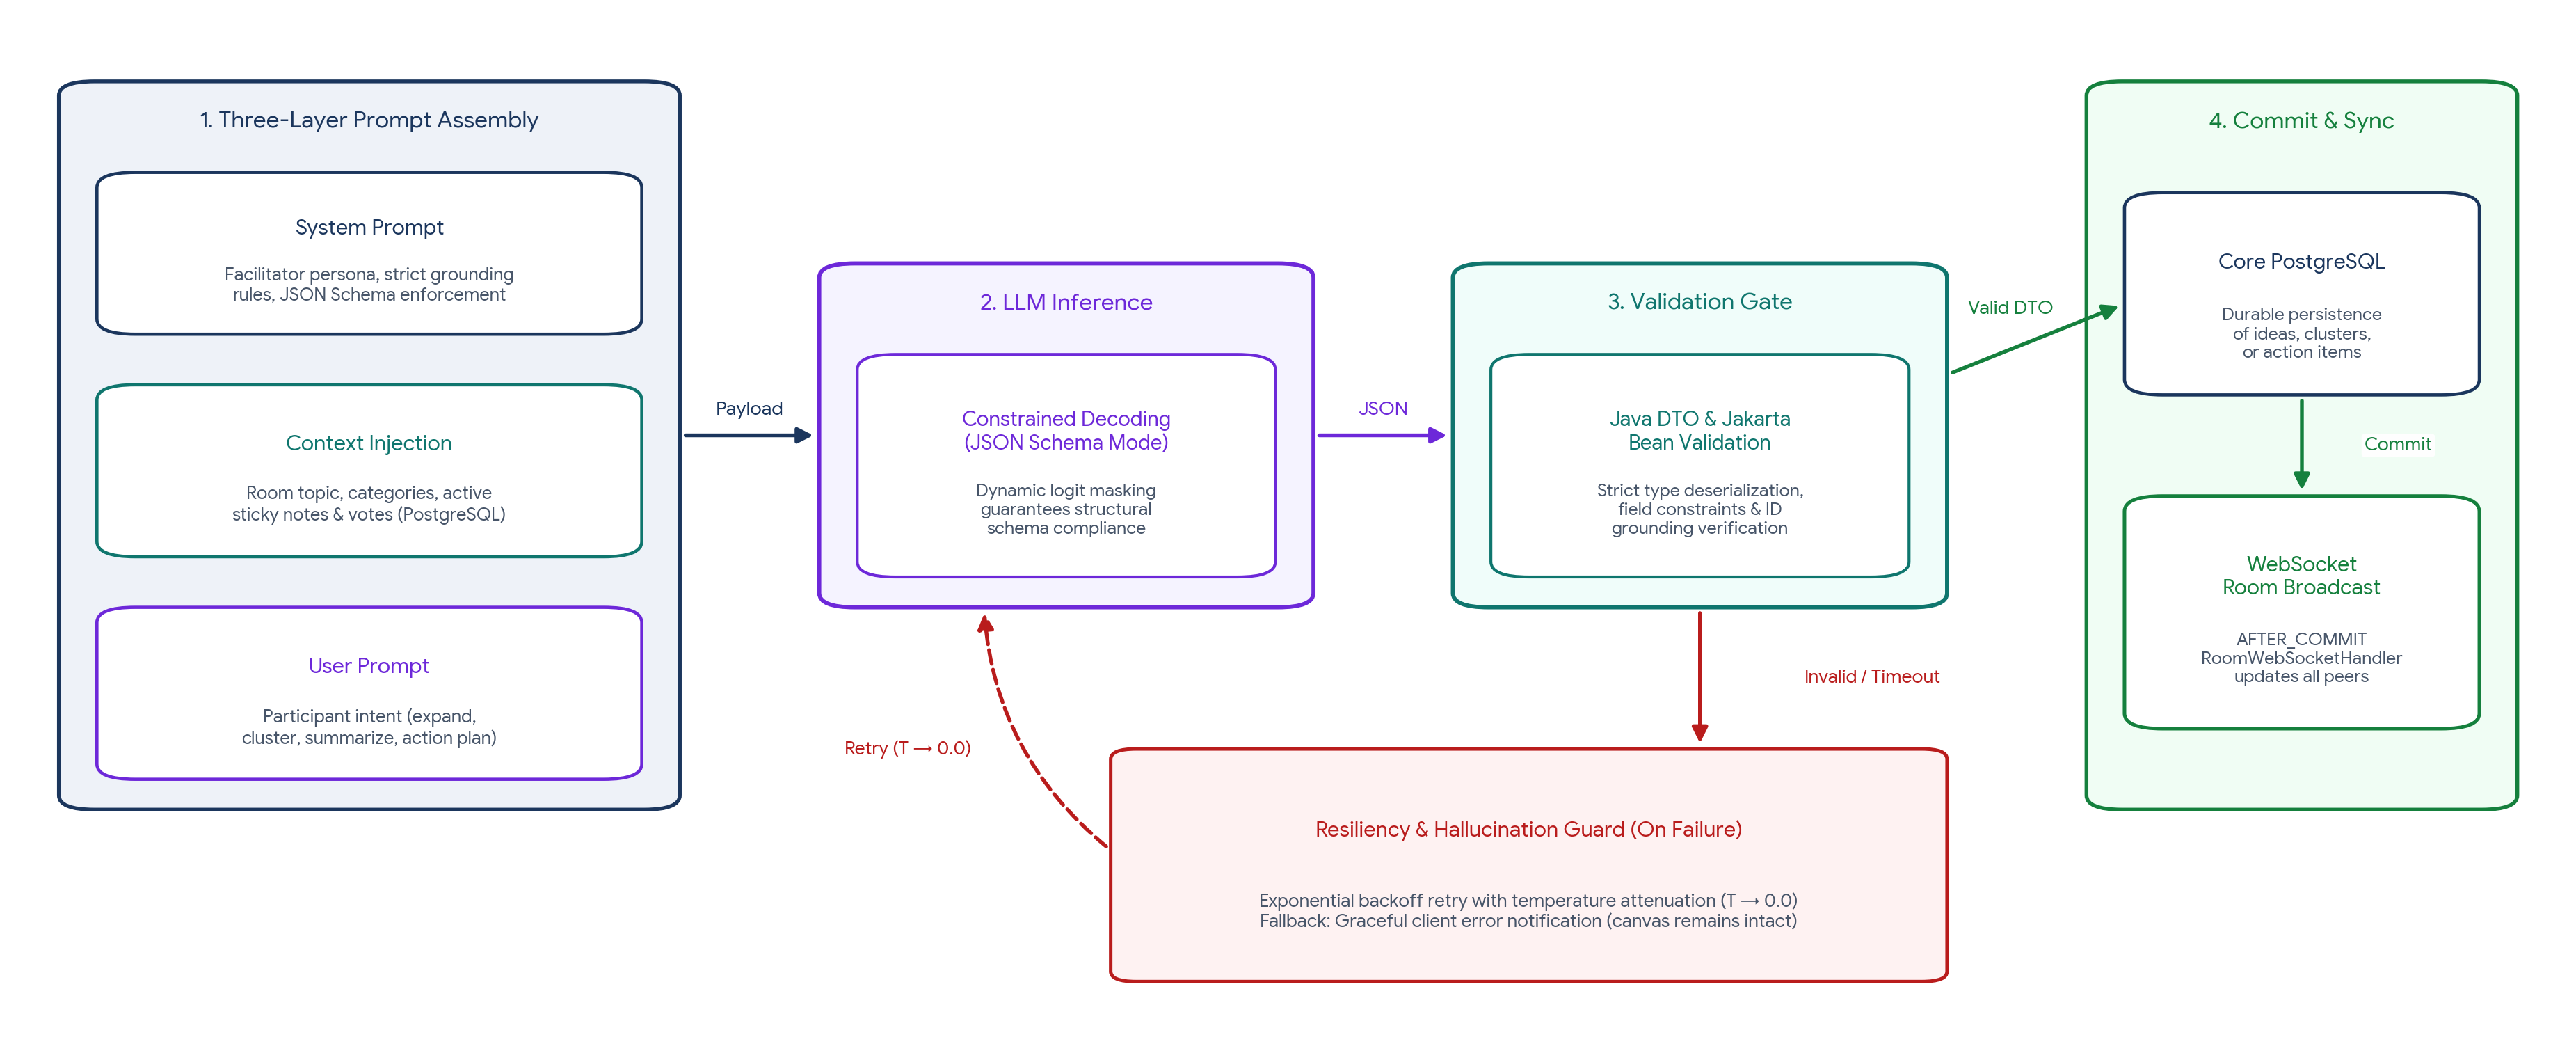
\includegraphics[width=0.9\textwidth]{fig-prompt-pipeline}
    \caption{Prompt engineering pipeline: system prompt, context injection, and user prompt feed the LLM, whose output is schema-validated before persistence and broadcast.}
    \label{fig:prompt-pipeline}
\end{figure}

\subsubsection{Structured Output Enforcement and JSON Schema Validation}
Collaborative platforms cannot reliably consume arbitrary natural language; updating sticky notes and creating categories requires deterministic, machine-readable data structures.
\begin{itemize}
    \item \textbf{Constrained Decoding / JSON Schema Mode:} Modern LLM APIs allow developers to supply a formal \textbf{JSON Schema}~\cite{json_schema_spec}. During token generation, logits are dynamically masked, guaranteeing that the output stream strictly satisfies the schema.
    \item \textbf{Application-Level Deserialization:} The incoming response must be deserialized into strongly-typed Java DTOs and validated using Jakarta / Hibernate Validator before persistence or WebSocket broadcast.
\end{itemize}

\subsubsection{Hallucination Mitigation and Resiliency Strategies}
LLMs are subject to \textbf{hallucinations}---generating plausible-sounding but factually ungrounded assertions~\cite{ji2023survey}. To mitigate hallucinations and guarantee system reliability, the target architecture incorporates:
\begin{itemize}
    \item \textbf{Grounding via Strict Context Windows:} Restricting the LLM to only reason over ideas explicitly passed in the prompt payload, with explicit instructions forbidding external speculation.
    \item \textbf{Retry and Fallback Mechanisms:} In the event of schema deserialization failure or API timeout, exponential backoff retries with temperature attenuation ($T \to 0.0$) must be executed, falling back to a graceful error notification rather than crashing the real-time canvas.
\end{itemize}


\section{SaaS Monetization \& Resource Governance}
\label{sec:saas_governance}

\subsection{SaaS Architectural Foundations}
Transitioning an ideation platform into a Software-as-a-Service (SaaS) commercial offering introduces critical architectural considerations regarding multi-tenancy, subscription lifecycles, and operational cost governance.

\subsubsection{Multi-Tenancy Isolation Models}
Multi-tenancy allows a single software instance to serve multiple distinct customer organizations (tenants). Three primary architectural patterns exist in cloud databases:
\begin{enumerate}
    \item \textbf{Database-per-Tenant:} Each tenant possesses a physically isolated database instance. While providing maximal data isolation and regulatory compliance, it incurs high infrastructure overhead and complex maintenance.
    \item \textbf{Schema-per-Tenant:} Tenants share a single database server but operate within dedicated relational schemas.
    \item \textbf{Shared Database, Shared Schema (Row-Level Isolation):} Tenants share the same database tables, with all entities partitioned via a tenant discriminator column (e.g., \texttt{tenant\_id}). This model offers maximum cost efficiency and horizontal scalability, but requires rigorous application-level or PostgreSQL Row-Level Security (RLS) policies to prevent cross-tenant data leakage.
\end{enumerate}

\subsubsection{Subscription Lifecycles and Tiering}
Commercial SaaS platforms operate tier-based subscription lifecycles governed by payment gateways (e.g., Stripe, LemonSqueezy). A tenant transitions through distinct states:
Trial $\rightarrow$ Active $\rightarrow$ Past Due $\rightarrow$ Canceled $\rightarrow$ Expired.
Access control middleware inspects tenant entitlement tokens on every API invocation, conditionally gating advanced functionality (e.g., unlimited rooms, export capabilities, AI assistants) based on the active plan tier.

\subsubsection{API Rate Limiting and AI Cost Governance}
In traditional web architectures, rate limiting protects servers against Denial of Service (DoS) attacks using algorithms such as the \textbf{Token Bucket} or \textbf{Leaky Bucket}. In AI-powered SaaS platforms, resource governance assumes an even more critical economic dimension: \textbf{AI Token Cost Governance}.

Because commercial LLM providers charge per thousand input and output tokens, unrestricted user access can lead to rapid financial exhaustion. Production SaaS platforms enforce multi-layered governance:
\begin{itemize}
    \item \textbf{Credit / Token Quotas:} Each tenant is allocated a monthly token budget according to their subscription tier.
    \item \textbf{Sliding-Window Rate Limits:} Restricting the number of AI requests per user per minute to prevent burst overuse.
    \item \textbf{Model Cascading / Dynamic Routing:} Routing simple requests to lightweight models (e.g., Gemini Flash-Lite) while reserving heavy frontier models for complex multi-idea synthesis.
\end{itemize}


\subsection{Resource Governance in the Current MindSpark Prototype}
\label{subsec:mindspark_saas_status}

In the current baseline implementation, \textbf{multi-tenancy, subscription tiers, payment gateways, and AI token quotas are not implemented}.

The verified codebase exhibits the following architectural state:
\begin{itemize}
    \item \textbf{Single-Tenant Relational Schema:} The database schema operates under a single shared namespace without \texttt{tenant\_id} columns on \texttt{Room}, \texttt{User}, or \texttt{Idea} entities. User identities are managed globally through a single Keycloak realm (\texttt{mindspark}).
    \item \textbf{Absence of Plan Tiers and Billing:} There are no subscription entities, credit balances, or payment webhooks in either backend or frontend services.
    \item \textbf{Implemented Transport Rate Limiting:} MindSpark does implement strict per-session rate limiting on the WebSocket transport layer in \texttt{RoomWebSocketHandler.java} (capping cursor updates to 25/s and card drags to 15/s) and limits concurrent sessions per user to 10 in \texttt{PresenceService.java}. However, these guards protect server memory and network throughput, rather than governing SaaS business quotas.
\end{itemize}
Designing and integrating a multi-tenant subscription framework and AI quota middleware remains a key objective for the platform's commercial roadmap.


\section{Conclusion}
\label{sec:conclusion}

This chapter has established the theoretical foundations, industry benchmarks, and technical state of the art essential for the development of MindSpark:
\begin{enumerate}
    \item \textbf{Collaborative Ideation:} Reviewed the psychological mechanics of group ideation, highlighting how digital platforms eliminate production blocking and analyzing the technical requirements for true anonymous voting to mitigate evaluation apprehension.
    \item \textbf{Real-Time Architecture:} Analyzed communication protocols, demonstrating that bidirectional WebSockets with normalized coordinates, soft-locking, and transaction-safe broadcasting provide the low-latency guarantees required for visual collaboration. The audit verified that MindSpark's core real-time infrastructure successfully implements these standards.
    \item \textbf{Comparative Benchmark:} Benchmarked MindSpark against Miro, Mural, Klaxoon, and FigJam using verified official pricing and feature documentation, identifying that commercial tools gate AI capabilities behind high subscription tiers.
    \item \textbf{Generative AI and Architecture:} Investigated Transformer mechanics, prompt engineering, and the confirmed \texttt{ai-service} microservice utilizing Google Gemini and Groq LPU routing. The audit established that while MindSpark currently features zero AI and billing implementation, the theoretical specifications formulated herein provide the precise blueprint for subsequent design and implementation chapters.
\end{enumerate}

Building on these insights, \textbf{Chapter 3 (System Analysis and Design)} will formalize the software requirements, domain modeling, and microservice architecture required to integrate the confirmed \texttt{ai-service} and anonymous voting engine directly into MindSpark's verified collaborative foundation.
